\section{Task: Import MySQL DB}
\label{sec:task_import_mysql_db}

This task allows importing of an exported SASS-C Verif job database (or other MySQL exported databases).

\begin{figure}[H]
  \hspace*{-2.5cm}
    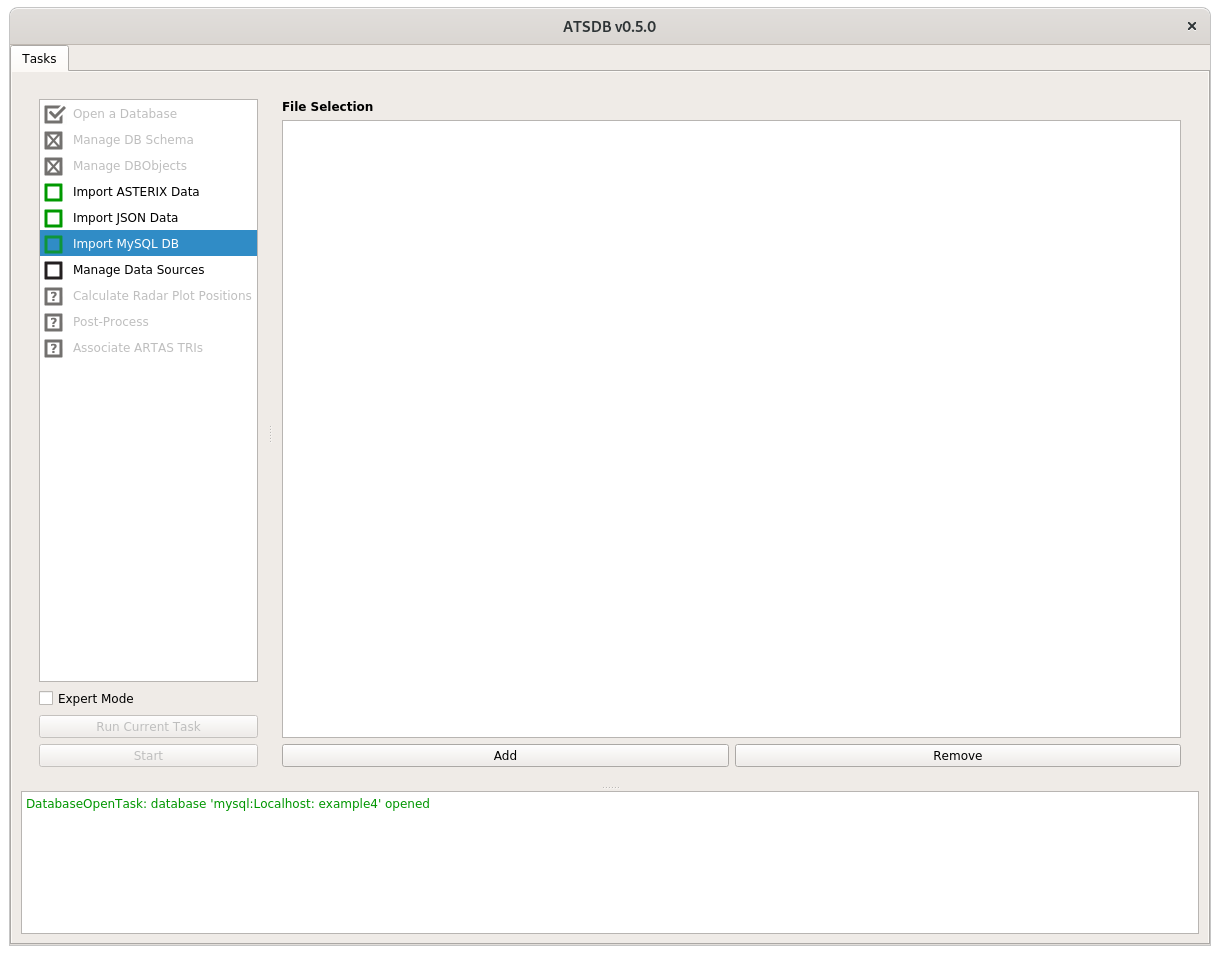
\includegraphics[width=19cm]{../screenshots/database_import.png}
  \caption{Task: Import MySQL database}
\end{figure}

\subsection{File Selection}

In the 'File Selection' list, a list of available database files is given. Entries can be added using the 'Add' button or removed using the 'Remove' buttons. Please note that either text files can be imported, or archives containing the same with the following formats: *.sql *.tar.gz *.gz *.tar *.tgz \\

Please add and select the file to be imported, after which the 'Run Current Task' button will become available. \\

\paragraph{Importing a MySQL Text File}

A previously exported MySQL database can be read from a text file and written into the current database. \\

Please note the following points:

\begin{itemize}  
\item The text file must contain valid MySQL statements
\item MySQL functions/views are not imported, only data which can be inspected
\item If more than 3 errors occur during the import process, it is aborted
\item If the import process was aborted, the current database might contain already imported parts which are not deleted automatically
\end{itemize}

\paragraph{Importing a MySQL Text Archive File}

A previously exported MySQL database can be read from a text archive file and written into the current database. \\

Please note the following points:

\begin{itemize}  
\item This function does \textbf{not} work to import an Verif-exported \textit{evaluation tgz}, but imports an \textit{SQL archive} from inside such an evaluation tgz
\item The text archive file must follow the same points as in the \textbf{Importing a MySQL Text File} section.
\item All files within the archive are read and imported into the database
\item If more than 3 errors occur during the import process, it is aborted
\item If the import process was aborted, the current database might contain already imported parts which are not deleted automatically
\end{itemize}

\paragraph{Importing a SASS-C Evaluation Export}

The following steps must be taken:\\

\begin{itemize}  
\item An export from a SASS-C evaluation must exist, e.g. 'example.tgz'
\item Using your favorite archive manager, extract the file 'tgz-tmp/<JOB\_NAME>/exported.sql.gz'
\item Select the previously extracted 'exported.sql.gz'
\end{itemize} 

\subsection{Runnning}

Using the 'Run Current Task' button the task can be performed. During import a status indication will be shown:

\begin{figure}[H]
  \center
    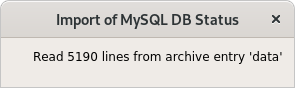
\includegraphics[width=6cm]{../screenshots/mysql_import_status.png}
  \caption{Import MySQL data task status}
\end{figure}

After an successful import, a confirmation will be shown as follows:

\begin{figure}[H]
  \center
    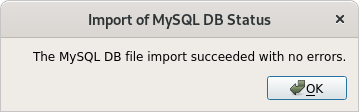
\includegraphics[width=6cm]{../screenshots/mysql_import_done.png}
  \caption{Import MySQL data task done}
\end{figure}
